%%%%%%%%%%%%%%%%%%%%%%%%%%%%%%%%%%%%%%%%%%%%%%%%%%%%%%%%%%%%%%%%%%%%%%%%
%%%  THIS TEX FILE IS TO GENERATE PDF FILE FOR 
%%% 
%%%  COPYRIGHT (C) JIMMY LIN, 2013, UT AUSTIN
%%%%%%%%%%%%%%%%%%%%%%%%%%%%%%%%%%%%%%%%%%%%%%%%%%%%%%%%%%%%%%%%%%%%%%%%
\documentclass[9pt]{beamer}
%%%%%%%%%%%%%%%%%%%%%%%%%%%%%%%%%%%%%%%%%%%%%%%%%%%%%%%%%%%%%%%%%%%%%%%%
%%%  PACKAGES USED IN THIS TEX SOURCE FILE
%%%%%%%%%%%%%%%%%%%%%%%%%%%%%%%%%%%%%%%%%%%%%%%%%%%%%%%%%%%%%%%%%%%%%%%%
\usepackage{graphicx}
\usepackage{wrapfig}
\usepackage{geometry}
\usepackage{color}
%\usepackage{JSPPT}
%%%%%%%%%%%%%%%%%%%%%%%%%%%%%%%%%%%%%%%%%%%%%%%%%%%%%%%%%%%%%%%%%%%%%%%%
%%% PRESENTATION INFORMATION
%%%%%%%%%%%%%%%%%%%%%%%%%%%%%%%%%%%%%%%%%%%%%%%%%%%%%%%%%%%%%%%%%%%%%%%%
\title{An Overview of Multiagent Systems}
\author[Jimmy Lin and Barry Feigenbaum]{\bf Jimmy Lin \\Barry Feigenbaum}
\institute{\bf Prof. Risto Miikkulainen\\[0.3cm] Department of Computer Science \\The University of Texas At Austin}

%%%%%%%%%%%%%%%%%%%%%%%%%%%%%%%%%%%%%%%%%%%%%%%%%%%%%%%%%%%%%%%%%%%%%%%%
%%% TITLE PAGE
%%%%%%%%%%%%%%%%%%%%%%%%%%%%%%%%%%%%%%%%%%%%%%%%%%%%%%%%%%%%%%%%%%%%%%%%
\begin{document}
\begin{large}
    \frame{\maketitle}%\titlepage
\end{large}

\frame{
    \frametitle{Table of Contents}
    \tableofcontents
}

%%%%%%%%%%%%%%%%%%%%%%%%%%%%%%%%%%%%%%%%%%%%%%%%%%%%%%%%%%%%%%%%%%%%%%%%
%%% DOCUMENTATION STARTS FROM HERE
%%%%%%%%%%%%%%%%%%%%%%%%%%%%%%%%%%%%%%%%%%%%%%%%%%%%%%%%%%%%%%%%%%%%%%%%
\section{Introduction}
\frame{
    \frametitle{Introduction and Motivation}
    good
}

\frame{
    \frametitle{Social Learning}
    \begin{columns}[T] 
             \begin{column}[T]{5cm} 
             \begin{itemize}
                 \item In \textbf{social learning}, agents improve their own performance by learning from observations made by other members of the population
                 \item Traditionally, agents are partitioned into students and teachers, where teachers are chosen to be high fitness members of the population
                 \item \textbf{Problem}: Fitness is not a guarantee of superior behavior. High fitness agents may make mistakes, and low fitness agents can still do well under certain circumstances
                 \end{itemize}
             \end{column}
             \begin{column}[T]{4cm} 
             	
\includegraphics[width=4.5cm]{images/social_learning.png}
             \end{column}
        \end{columns}
}

\frame{
    \frametitle{Cooperative search}
    \begin{columns}[T] 
             \begin{column}[T]{4cm} 
             \begin{itemize}
                \item In this example, agents represent \textbf{Unmanned Aerial Vehicles} (\textbf{UAVs}) searching a grid of airspace 
                \item Agents have limited communication and some mobility restrictions (such as slow turning)
             \end{itemize}
             \end{column}
             \begin{column}[T]{6.5cm} 
             	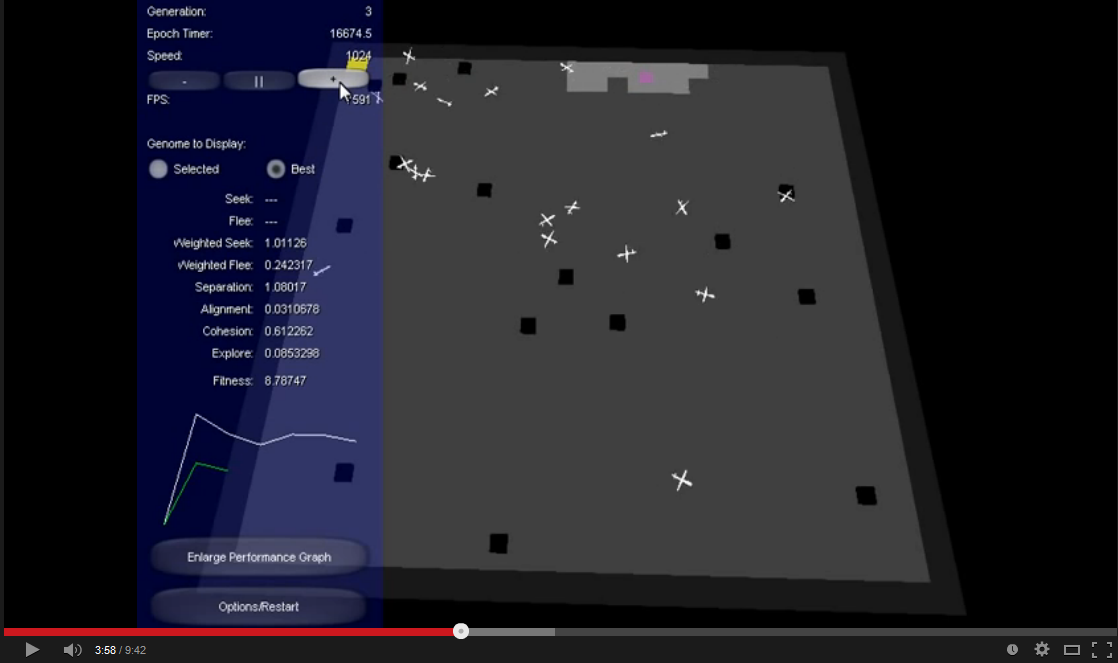
\includegraphics[width=7cm]{images/uav/youtube.png}
             \end{column}
        \end{columns}
}

\frame{
    \frametitle{UAV Example: Goals}
    \begin{columns}[T] % contents are top vertically aligned
         \begin{column}[T]{5cm} % each column can also be its own environment
         \begin{itemize}
             \item Compare a \textit{centralized} approach, where agents share a network, to a \textit{decentralized} approach
             \item Determine whether opportunistic sharing of network weights improves the speed and accuracy of learning
         \end{itemize}
         \end{column}
         \begin{column}[T]{6cm} % alternative top-align that's better for graphics
              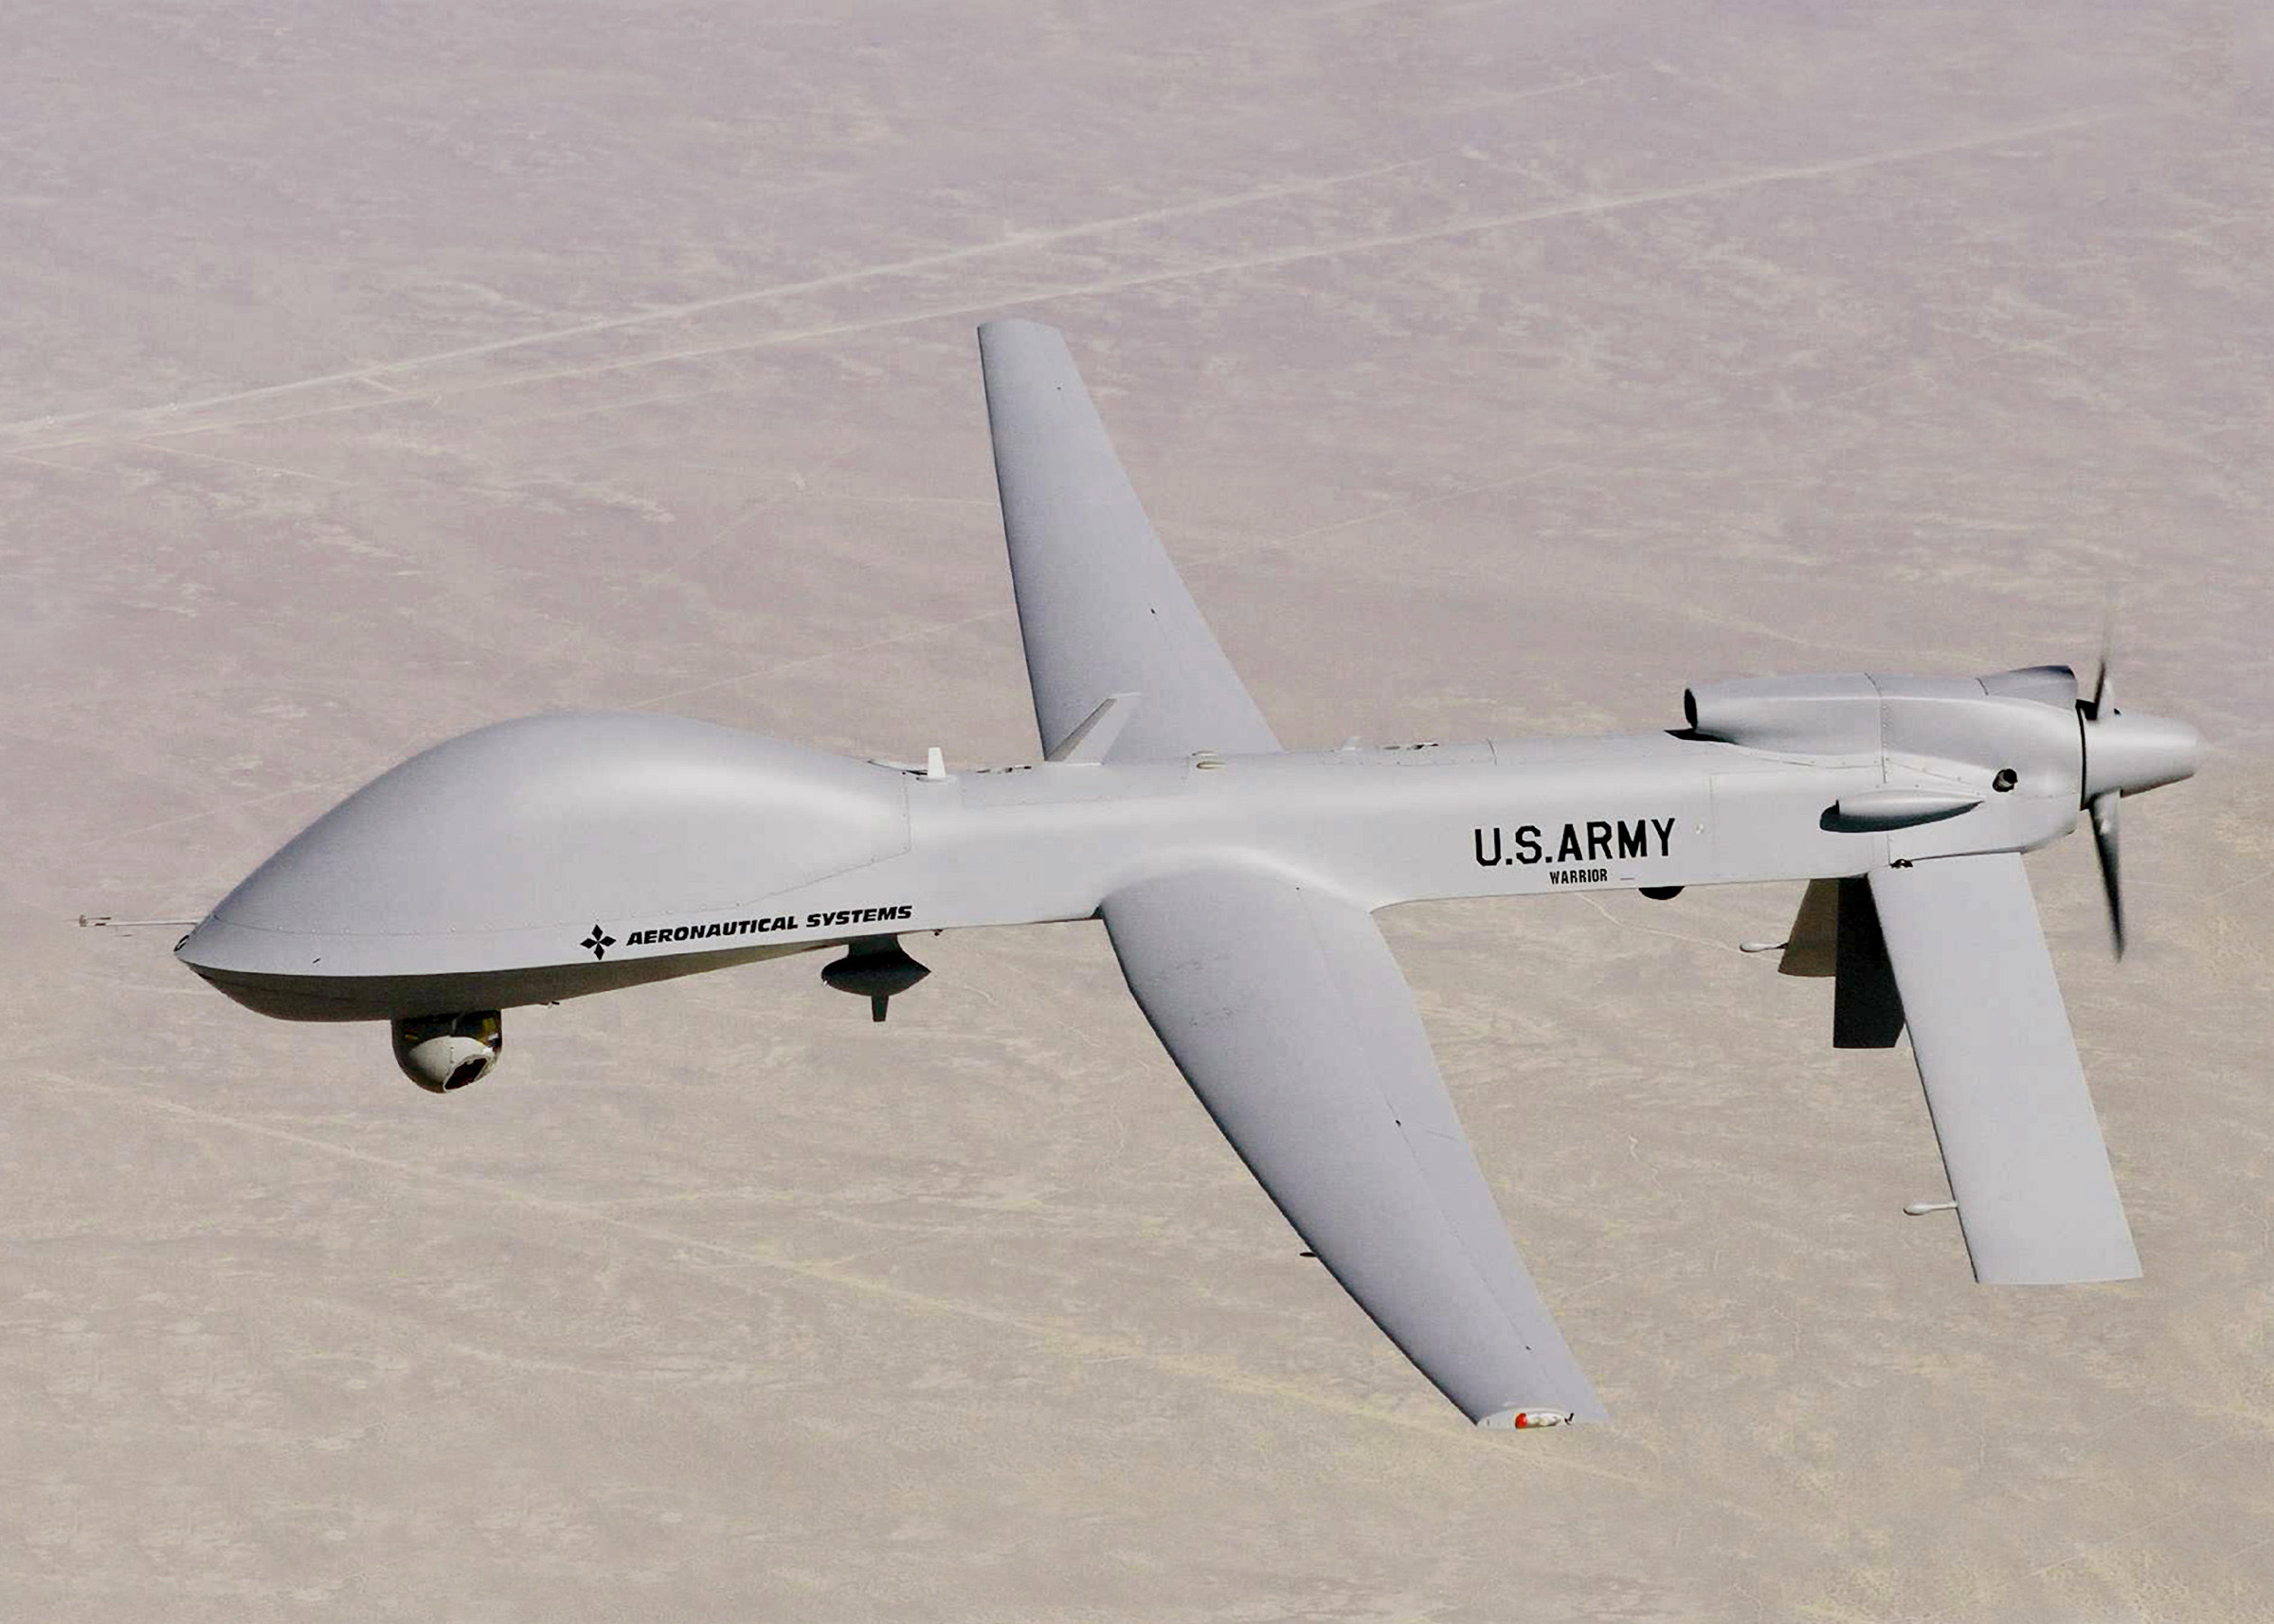
\includegraphics[width=6cm]{images/uav/UAV_Drone.jpg}
         \end{column}
    \end{columns}
    
}

\frame{
    \frametitle{UAV Example: Setup}
    \begin{columns}[T] 
    	\begin{column}[T]{5cm} 
		    \begin{itemize}
		    \item Trained via Reinforcement Learning
		    \item The search space is divided into a grid, and each cell is given a \textit{certainty} value between 0 and 1 
		    \item The uncertainty of a cell is reduced by half for each agent that enters that cell
		    \item Rewards equal the decrease in uncertainty in a given cell divided evenly among the entering agents 
		    \end{itemize}
		\end{column}
		\begin{column}[T]{5cm}
			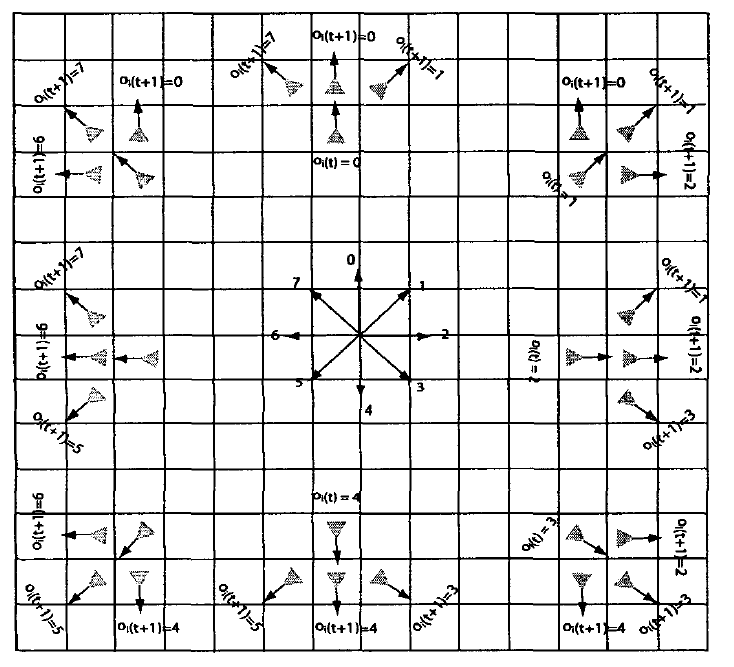
\includegraphics[width=5.5cm]{images/uav/overview.png}
		\end{column}
	\end{columns}
}

\frame{
    \frametitle{UAV Example}
    \begin{itemize}
    \item Agents want to spread out and avoid entering the same cell
    \item At each time-step, an agent only has three options (turn left, turn right, keep straight)
    \item Three neural networks are used to estimate the benefit of each course
    \end{itemize}
    Compare three architectures:
	\begin{itemize}
	\item \textbf{Centralized Learning}: three shared networks receive input from all agents
	\item \textbf{Decentralized Learning}: each agent has it's own three networks
	\item \textbf{Opportunistic Cooperative Learning}: each agent has it's own three networks. Additionally, when two agents come close together, the less successful one copies the other's network with probability $\pi$
	\end{itemize}
}

\frame{
    \frametitle{UAV Example: Results}
    \begin{center}
    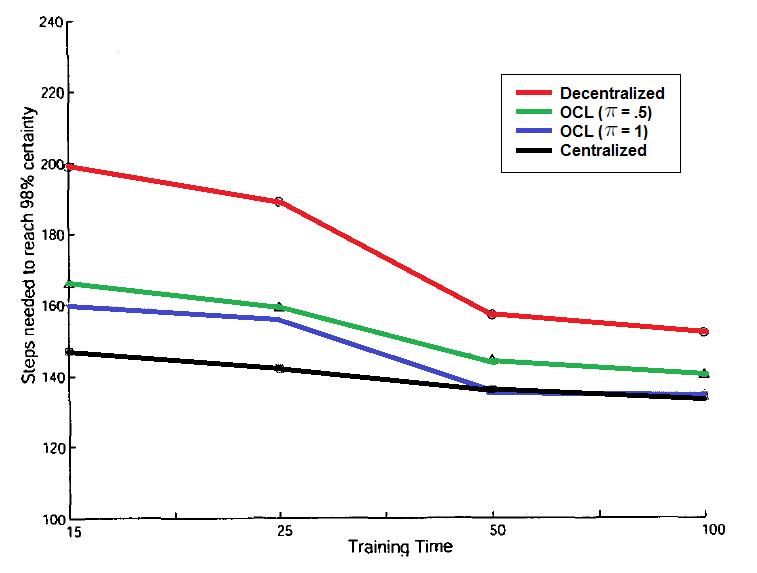
\includegraphics[height=7cm]{images/uav/results_color.png}
    \end{center}
    
}

\frame{
    \frametitle{Egaltarian Social Learning}
    \begin{itemize}
    \item In \textbf{Egaltarian Social Learning} (\textbf{ESL}), agents learn from each other instead of from a limited number of teachers 
    \item The population of agents is partitioned into subcultures at the start of each generation
    \item An agent may probabilistically learn from any other agent in the same subculture
    %\item An agent's quality as an example is determined by the receiving agent
    \end{itemize}
}

\frame{
    \frametitle{ESL Example: Foraging}
    \begin{itemize}
    \item Agents move independently across a continuous world filled with several types of plants
    \item Plants are automatically consumed when an agent draws close enough; some types of plant give positive reward, others negative reward
    \item Agents have sensors for each type of plant, as well as a sensor for their own velocity
    \item They cannot see other agents, or plants they have already consumed
    \item Networks are trained with backpropagation and NeuroEvolution of Augmenting Topologies (NEAT)
    \end{itemize}
}

\frame{
    \frametitle{ESL Example: Foraging (Results)}
    \begin{columns}[T] % contents are top vertically aligned
         \begin{column}[T]{4cm} % each column can also be its own environment
         \begin{itemize}
             \item ESL without subcultures performs worse than plain neuroevolution
             \item Adding subcultures results in a significant improvement
         \end{itemize}
         \end{column}
         \begin{column}[T]{6cm} % alternative top-align that's better for graphics
              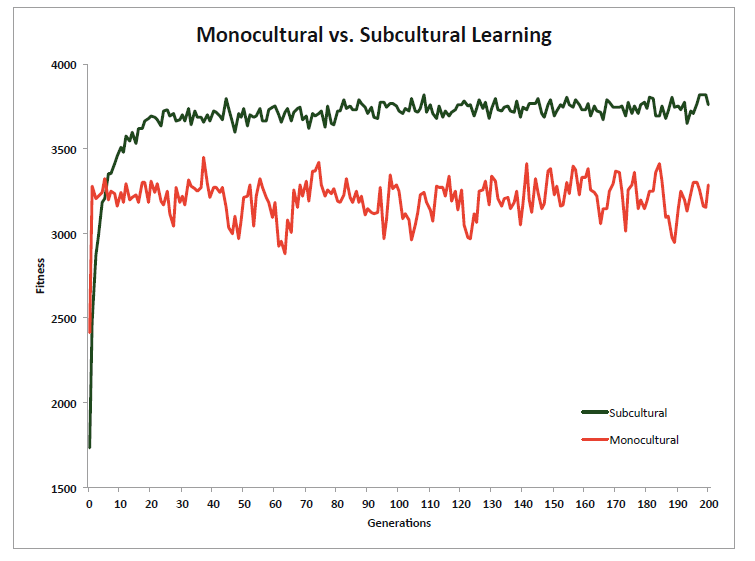
\includegraphics[height=5cm]{images/foraging/monocultural_vs_subcultural.png}
         \end{column}
    \end{columns}
    
}

\frame{
    \frametitle{ESL Example: Foraging (Results)}
    Comparing ESL with student-teacher learning and plain neuroevolution
    \begin{columns}[T] 
         \begin{column}[T]{4.5cm} 
         	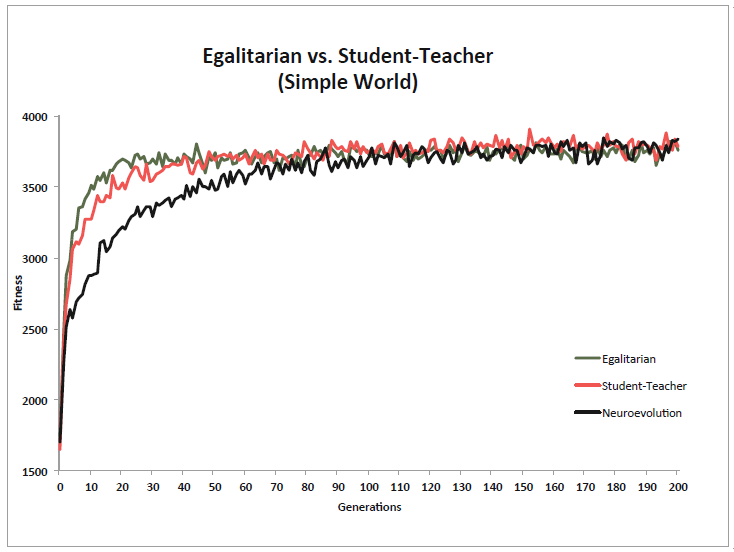
\includegraphics[height=4.2cm]{images/foraging/student_teacher_simple.png}
         	
         	Simple environment (few plant types)
         \end{column}
         \begin{column}[T]{4.5cm} 
           	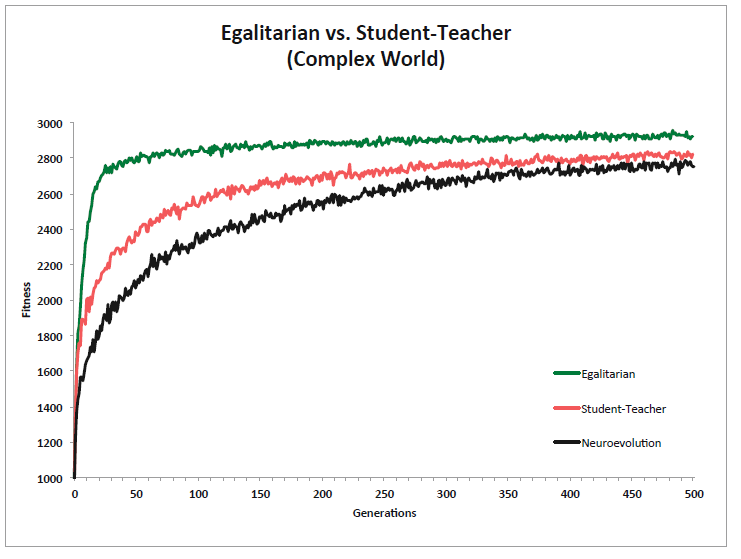
\includegraphics[height=4.2cm]{images/foraging/student_teacher_complex.png}
           	
           	Complex environment (many plant types)
         \end{column}
    \end{columns}
}

\frame{
    \frametitle{ESL Example: Foraging (Conclusion)}
    \begin{itemize}
    \item ESL is advantageous because it promotes diversity and avoids premature convergence
    \end{itemize}
}

\frame{
    \frametitle{Communication}
     
}

\frame{
    \frametitle{Predator / Prey}
    \begin{columns}[T] 
        \begin{column}[T]{5cm}
			Three different examples:
		  	\begin{itemize}
		  	\item Centralized network
		  	\item Autonomous networks with communication
		  	\item Autonomous networks \textit{without} communication
		  	\end{itemize}
		  	All are trained using ESP or \textbf{Multi-Agent ESP} 
	  	\end{column}
	  	\begin{column}[T]{6cm}
			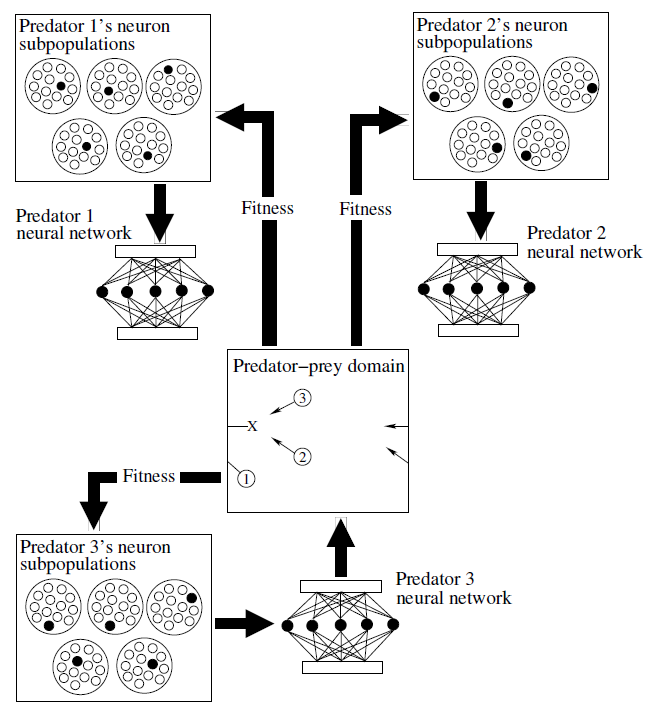
\includegraphics[width=5.5cm]{images/predator_prey/multiagent_esp.png}
	  	\end{column}
	\end{columns}
}

\frame{
    \frametitle{Centralized Network}
    \begin{center}
    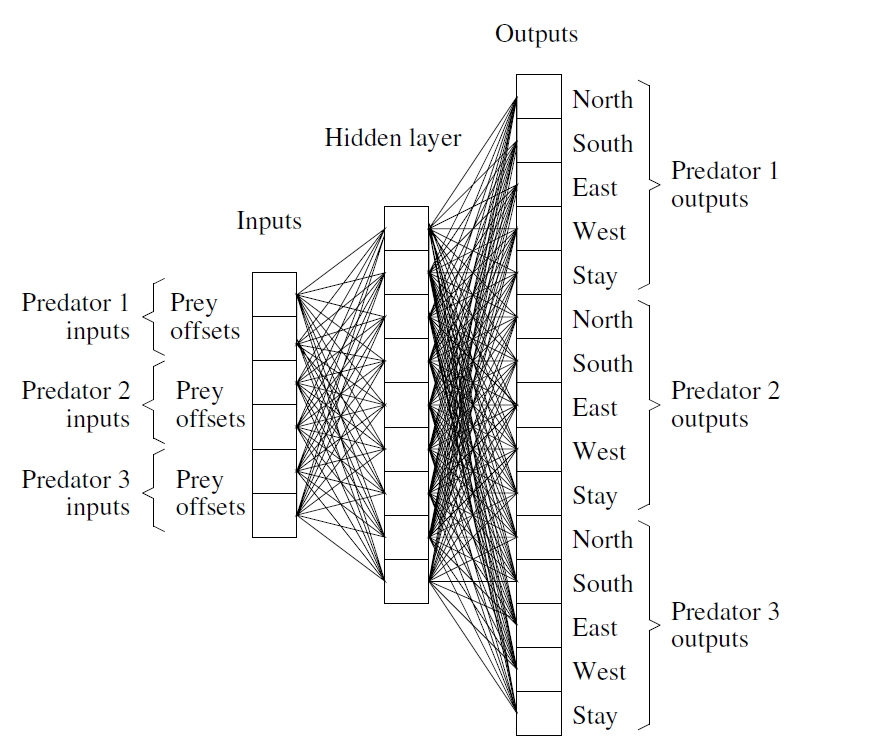
\includegraphics[width=9cm]{images/predator_prey/central_network.png}
    \end{center}
}

\frame{
    \frametitle{Communicating Network}
    \begin{center}
    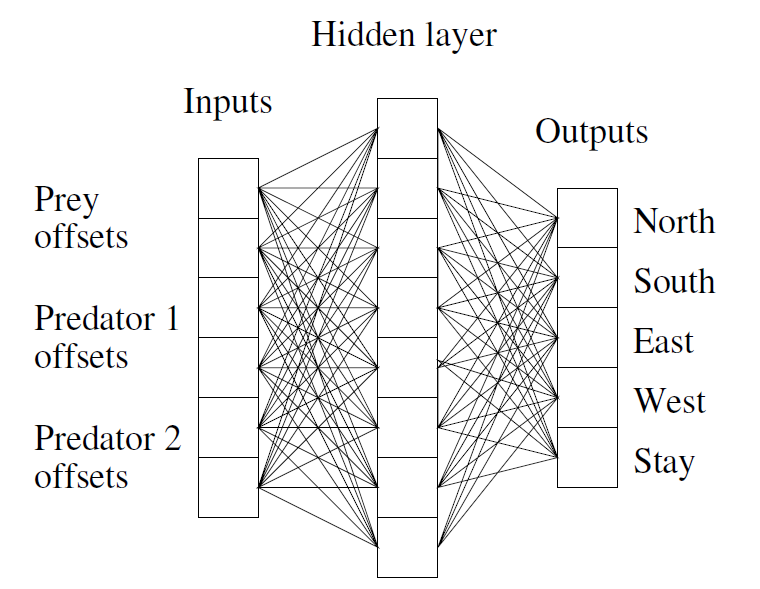
\includegraphics[width=8cm]{images/predator_prey/communication_network.png}
    \end{center}
}

\frame{
    \frametitle{Non-communicating Network}
    \begin{center}
    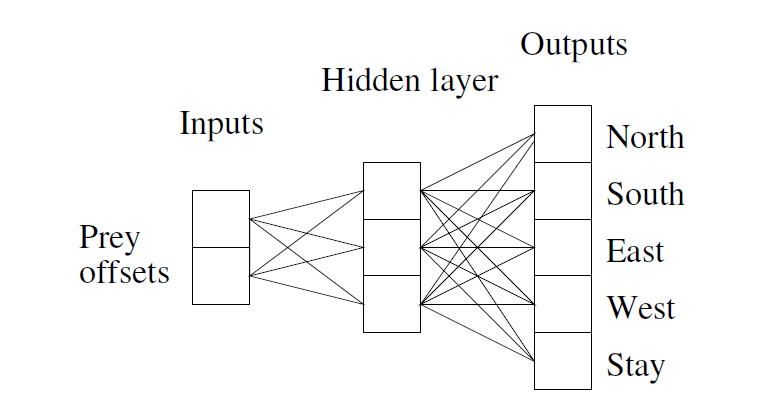
\includegraphics[width=8cm]{images/predator_prey/noncommunication_network.png}
    \end{center}
}

\frame{
    \frametitle{Predator / Prey Results}
    How long does it take these networks to become successful?
    \begin{columns}[T] 
         \begin{column}[T]{6cm} 
         	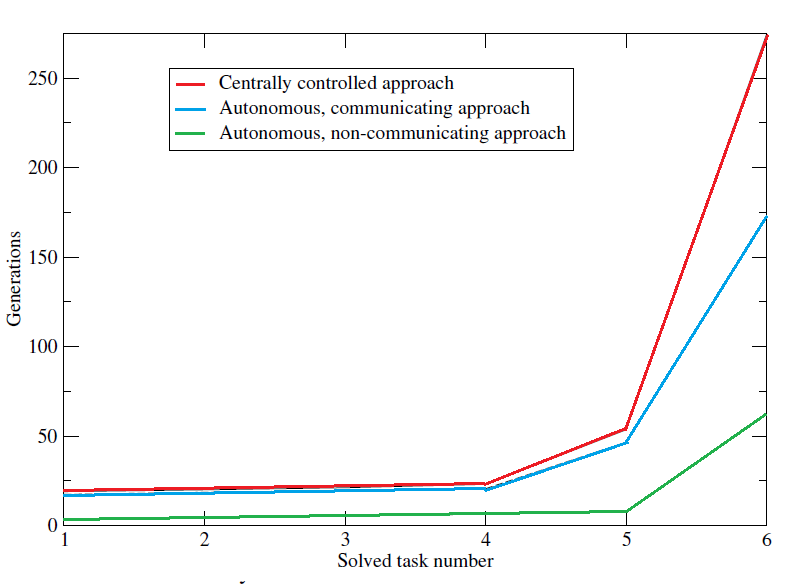
\includegraphics[height=4.5cm]{images/predator_prey/results_line.png}
         	\begin{center}
         	\end{center}
         \end{column}
         \begin{column}[T]{6cm} 
           	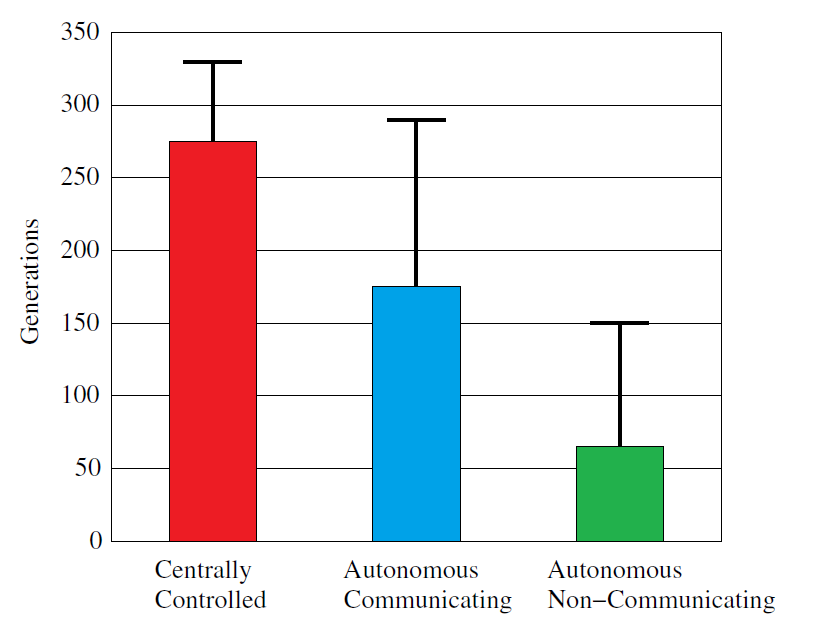
\includegraphics[height=4.5cm]{images/predator_prey/results_bar.png}
           	\begin{center}
           	\end{center}
         \end{column}
    \end{columns}
    \textbf{Conclusion}: The predators are able to cooperate using \textbf{stigmergy} -- indirect coordination based on the environment
    \begin{itemize}
    \item What if the environment is more complicated?
    \end{itemize}  
}

\frame{
    \frametitle{Predator / Prey Conclusion}
    \begin{itemize}
    \item What happens if we use homogeneous networks? (All predators have the same network weights)
    \item Communication becomes a necessity
    \end{itemize}
    \begin{center}
    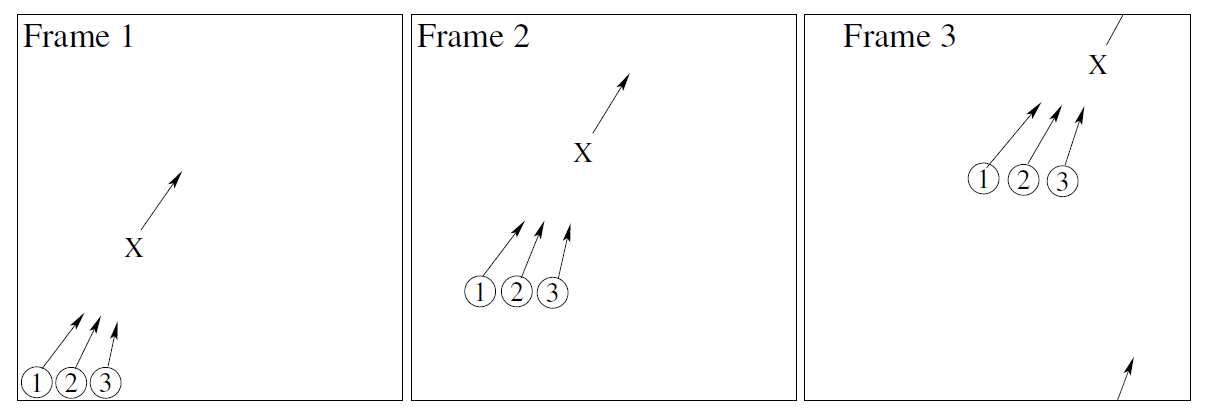
\includegraphics[width=9cm]{images/predator_prey/no_cooperation.png} 
    \end{center}
    \begin{itemize}
    \item Even with communication, homogeneous networks do poorly, catching the prey only 3\% of the time
    \end{itemize} 
}

\frame{
    \frametitle{Homogeneous Networks}
    \begin{itemize}
    \item Thus far, all multi-agent solutions have used heterogeneous networks
    \item In the predator prey, homogeneous networks performed very poorly
    \item Can we evolve agents with identical networks, which nevertheless cooperate by adopting different strategies?
    \end{itemize}
}

\frame{
    \frametitle{Legion Game}
    \begin{columns}[T] 
         \begin{column}[T]{4cm} 
         	The Legion game consists of:
         	\begin{itemize}
         	\item A hexagonal grid (the countryside)
         	\item A number of randomly placed cities
         	\item Several legions (defenders)
         	\item Many barbarian attackers
         	\end{itemize}
         	At every game tick, legions are penalized for each barbarian on the board
         \end{column}
         \begin{column}[T]{7cm} 
           	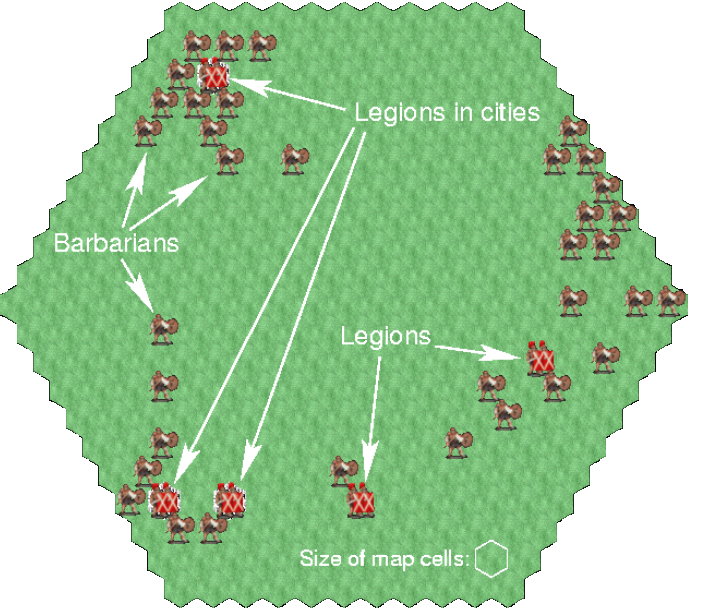
\includegraphics[height=6cm]{images/legion/setup.png}
         \end{column}
    \end{columns}
}

\frame{
    \frametitle{Legion Network}
    \begin{itemize}
    \item Each legion has six sensors for each of the six directions
    \item Can detect immediate adjacency as well as long-distance
    \end{itemize}
    \begin{columns}[T] 
         \begin{column}[T]{5.5cm} 
         	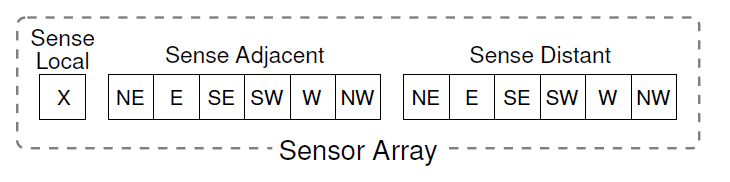
\includegraphics[width=6cm]{images/legion/inputs.png}
         	
         	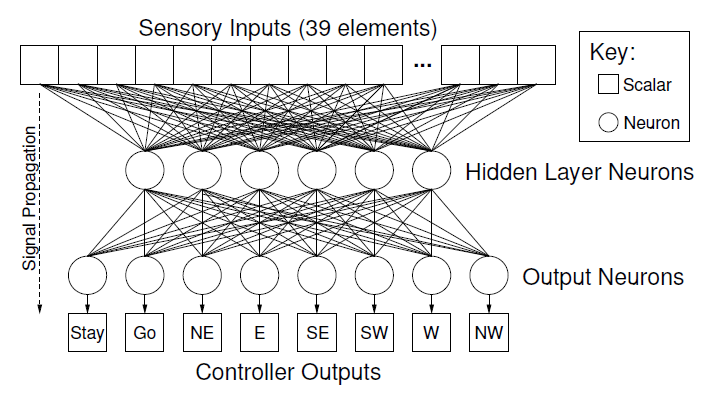
\includegraphics[width=6cm]{images/legion/network.png}
         \end{column}
         \begin{column}[T]{4.5cm} 
           	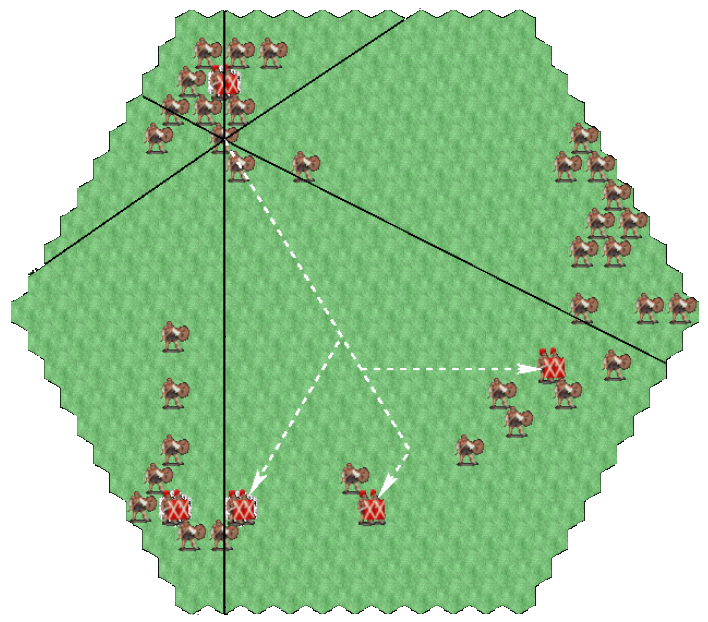
\includegraphics[width=5cm]{images/legion/sensors.png}
         \end{column}
    \end{columns}
}

\frame{
    \frametitle{Legion Results}
    \begin{itemize}
    \item Legions were trained with ESP neuroevolution
    \item Successfully learned to divide labor between "guard duty" and search and destroy" behavior
    \end{itemize}
    
    \begin{columns}[T] 
         \begin{column}[T]{5cm} 
         	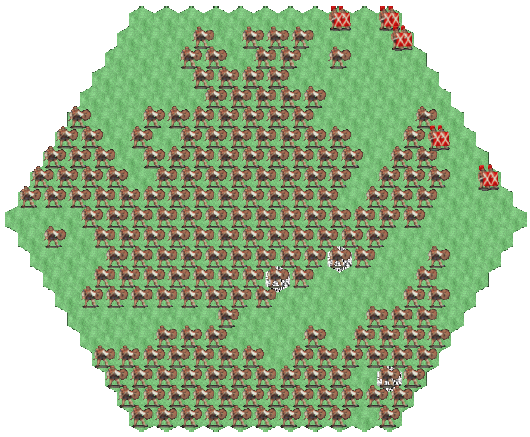
\includegraphics[width=5cm]{images/legion/before.png}
         	\begin{center}
         	Before training 
         	\end{center}
         \end{column}
         \begin{column}[T]{5cm} 
           	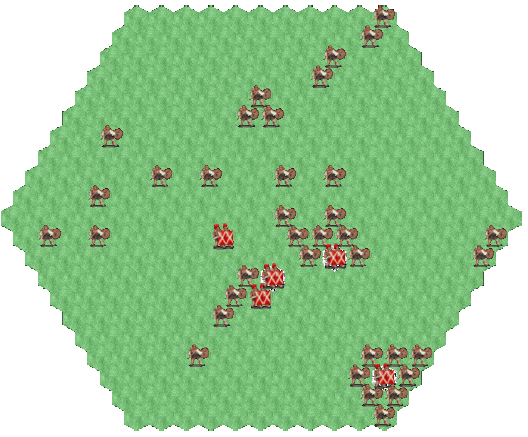
\includegraphics[width=5cm]{images/legion/after.png}
           	\begin{center}
           	After training 
           	\end{center}
         \end{column}
    \end{columns}
}

%%%%%%%%%%%%%%%%%%%%%%%%%%%%%%%%%%%%%%%%%%%%%%%%%%%%%%%%%%%%%%%%%%%%%%%%
%%% REFERENCES
%%%%%%%%%%%%%%%%%%%%%%%%%%%%%%%%%%%%%%%%%%%%%%%%%%%%%%%%%%%%%%%%%%%%%%%%
\section{References}
\frame{
    \frametitle{References}
    \begin{thebibliography}{9}
        \bibitem{ConcreteMath} Liu, Tie, et al. "Learning to detect a salient object."\textit{ Computer Vision and Pattern Recognition, 2007. CVPR'07. IEEE Conference on. IEEE, 2007. }
    \end{thebibliography}
}
\end{document}
